\documentclass[a4paper, article, oneside, twocolumn, 10pt, USenglish, hidelinks]{memoir}

% Drawing
\usepackage{pgf,tikz}
\usetikzlibrary{arrows}


%% Encoding
\usepackage[utf8]{inputenc}
\usepackage[T1]{fontenc}


%% Color
\usepackage{xcolor}
\definecolor{title_color}{HTML}{333370}
\definecolor{todoback}{HTML}{E9E9F8}


%% Fonts and typography
%\usepackage{lmodern}           % Latin Modern Roman
\usepackage[scaled]{beramono}  % Bera Mono (Bitstream Vera Sans Mono)
%\renewcommand{\sfdefault}{phv} % Helvetica
\usepackage[final]{microtype}  % Improved typography
\usepackage{caladea}

\pretitle{\begin{center}\color{title_color}\huge\sffamily}                    % Title
\renewcommand{\abstractnamefont}{\color{title_color}\sffamily\bfseries}                 % Abstract
\renewcommand*{\chaptitlefont}{\color{title_color}\Large\sffamily\raggedright} % Chapter
\setsecheadstyle{\color{title_color}\Large\sffamily\raggedright}               % Section
\setsubsecheadstyle{\color{title_color}\large\sffamily\raggedright}          		    % Subsection


%% small gap between paragraphs
\setlength{\parskip}{2pt}


%% todo notes
\usepackage[color=todoback]{todonotes}


%% Style figures
\usepackage{caption}
\captionsetup{labelfont=bf}


%% Increase spacing before section and chapter titles
\makeatletter
\let\origchapter\chapter
\renewcommand\chapter{\@ifstar{\starchapter}{\nostarchapter}}

\newcommand\nostarchapter[1]
{\chapterprelude\origchapter{#1}\chapterpostlude}

\newcommand\starchapter[1]
{\chapterprelude\origchapter*{#1}\chapterpostlude}

\newcommand\chapterprelude{%
	\vspace{2.5em}
}

\newcommand\chapterpostlude{%
	%	\vspace{-1.4em}
}
\let\origsection\section
\renewcommand\section{\@ifstar{\starsection}{\nostarsection}}

\newcommand\nostarsection[1]
{\sectionprelude\origsection{#1}\sectionpostlude}

\newcommand\starsection[1]
{\sectionprelude\origsection*{#1}\sectionpostlude}

\newcommand\sectionprelude{%
	\vspace{1.5em}
}

\newcommand\sectionpostlude{%
%	\vspace{-1.4em}
}
\let\origsubsection\subsection
\renewcommand\subsection{\@ifstar{\starsubsection}{\nostarsubsection}}

\newcommand\nostarsubsection[1]
{\subsectionprelude\origsubsection{#1}\subsectionpostlude}

\newcommand\starsubsection[1]
{\subsectionprelude\origsubsection*{#1}\subsectionpostlude}

\newcommand\subsectionprelude{%
	\vspace{0.5em}
}

\newcommand\subsectionpostlude{%
	%	\vspace{-1.4em}
}
\makeatother


%% Mathematics
\usepackage{amssymb}   % Extra symbols
\usepackage{amsthm}    % Theorem-like environments
\usepackage{thmtools}  % Theorem-like environments
\usepackage{mathtools} % Fonts and environments for mathematical formuale
\usepackage{mathrsfs}  % Script font with \mathscr{}


%% Miscellanous
\usepackage{graphicx}  % Tool for images
\usepackage{babel}     % Automatic translations
\usepackage{csquotes}  % Quotes
\usepackage{textcomp}  % Extra symbols
\usepackage{lipsum}


%% Bibliography
\usepackage[backend = biber, style = alphabetic]{biblatex}
\addbibresource{oppgave_biblio.bib}


%% Cross references
\usepackage{varioref}
\usepackage{hyperref}
\urlstyle{sf}
\usepackage[nameinlink, capitalize, noabbrev]{cleveref}


%% Theorem-like environments
\declaretheorem[style = plain, numberwithin = chapter]{theorem}
\declaretheorem[style = plain,      sibling = theorem]{corollary}
\declaretheorem[style = plain,      sibling = theorem]{lemma}
\declaretheorem[style = plain,      sibling = theorem]{proposition}
\declaretheorem[style = definition, sibling = theorem]{definition}
\declaretheorem[style = definition, sibling = theorem]{example}
\declaretheorem[style = remark,    numbered = no]{remark}


%% Numbering within chapter
\counterwithin{equation}{chapter}
\counterwithin{figure}{chapter}

%% numbering of algorithms
\usepackage[chapter]{algorithm}


%% Operators
\DeclareMathOperator{\im}{im}
\DeclareMathOperator{\rank}{rank}
\DeclareMathOperator{\nul}{Nul}							% matrix-stuf
\DeclareMathOperator{\rref}{rref}
\DeclareMathOperator{\col}{Col}
\DeclareMathOperator{\row}{Row}
\newcommand{\inner}[2]{\langle #1 , #2 \rangle}
\DeclareMathOperator{\supp}{supp}


\newcommand{\minimize}[1]{\underset{#1}{\text{minimize}}~}
\newcommand{\maximize}[1]{\underset{#1}{\text{maximize}}~}
\newcommand{\subjectto}{\quad\subjto~}
\DeclareMathOperator*{\subjto}{subject~to}


%% New commands for sets
\newcommand{\N}{\mathbb{N}}   % Natural numbers
\newcommand{\Z}{\mathbb{Z}}   % Integers
\newcommand{\Q}{\mathbb{Q}}   % Rational numbers
\newcommand{\R}{\mathbb{R}}   % Real numbers
\newcommand{\Cx}{\mathbb{C}}   % Complex numbers

\newcommand{\K}{\mathbb{K}}   % R or C 
\renewcommand{\P}{\mathbb{P}} % Projective space
\newcommand{\indexset}[1]{\set{1, 2, \ldots, #1}}

%% New symbols
\renewcommand{\epsilon}{\varepsilon}


%% New commands for vectors
\renewcommand{\a}{\mathbf{a}}
\renewcommand{\b}{\mathbf{b}}
\renewcommand{\c}{\mathbf{c}}
\renewcommand{\v}{\mathbf{v}}
\renewcommand{\u}{\mathbf{u}}
\newcommand{\w}{\mathbf{w}}
\newcommand{\x}{\mathbf{x}}
\newcommand{\y}{\mathbf{y}}
\newcommand{\z}{\mathbf{z}}
\newcommand{\0}{\mathbf{0}}
\newcommand{\1}{\mathbf{1}}
\newcommand{\A}{\mathbf{A}}   % sensing matrix


% more math functions and symbols
\newcommand{\abs}[1]{\left|#1\right|}					% absulute value (singe line norm): | |
\newcommand{\ans}[1]{\underline{\underline{~#1~}}}		% two lines (for answers)
\newcommand{\sqrtl}[1]{\sqrt{#1~}}						% sqrt with longer line (nice for big equations)
\newcommand{\der}[2]{\frac{d}{d#2}\left(#1\right)}		% derivative
\newcommand{\norm}[1]{\lVert#1\rVert}					% double line norm: || ||
\newcommand{\bigo}{\mathcal{O}}							% Big-O notation

\newcommand{\twopartdef}[4]{							% for two-part definitions of functions, etc
	\left\{
	\begin{array}{cl}
		#1 & #2 \\
		#3 & #4
	\end{array}
	\right.
}
\newcommand{\threepartdef}[6]{							% for three-part definitions of functions, etc
	\left\{
	\begin{array}{cl}
		#1 & #2 \\
		#3 & #4 \\
		#5 & #6
	\end{array}
	\right.
}

\newenvironment{subdef}{
	\vspace{-4pt}
	\begin{enumerate}[label=\itshape(\roman*),leftmargin=2\parindent]
		\setlength{\itemsep}{4pt}
		\setlength{\parskip}{0pt}
		\setlength{\parsep}{0pt}
	}{\end{enumerate}}

\newcommand{\for}{\text{~~for }}
\newcommand{\all}{\text{all }}

\newcommand{\E}[1]{E\left[#1\right]}					% Statistics: Expectation, variance, gamma-function and probability
\newcommand{\var}[1]{\text{Var}\left[#1\right]}
\newcommand{\gam}[1]{\Gamma\left(#1\right)}
\newcommand{\pr}[1]{\text{Pr}\left(#1\right) }
\newcommand{\independent}{~{\perp\!\!\!\perp}~}
\newcommand{\iid}{\stackrel{iid}{\sim}}

\newcommand{\tuple}[1]{\langle #1 \rangle}				% tuples, sets..
\newcommand{\set}[1]{\{#1\}}
\newcommand{\st}{~|~}

\newcommand{\dB}{\text{\;dB}}							% enheter
\newcommand{\hz}{\text{\;Hz}}
\newcommand{\rads}{\;\text{rad}/\text{s}}

\DeclareMathOperator*{\argmin}{arg\,min}
\DeclareMathOperator*{\argmax}{arg\,max}

%% Miscellanous
%\renewcommand{\qedsymbol}{\(\blacksquare\)}
\usepackage{ifdraft}
\usepackage{enumitem}

\makeatletter
\renewcommand\footnoterule{%
	\kern-3\p@
	\hrule\@width \columnwidth
	\kern2.6\p@}
\makeatother

\tolerance = 5000 % LaTeX er normalt streng når det gjelder linjebrytingen.
\hbadness = \tolerance % Vi vil være litt mildere, særlig fordi norsk har så
\pretolerance = 2000 % mange lange sammensatte ord.s

\newcommand{\inputPone}{\begin{equation}
	\minimize{\mathbf{z} \in \Cx^{N}} \norm{\mathbf{z}}_1
	\subjectto \mathbf{A}\mathbf{z} = \mathbf{y}
	\tag{P$_1$}
	\end{equation}}


\title{Face Recognition with Compressive Sensing}
\author{Mathias Lohne}
\date{Spring, 2017}

\setcounter{topnumber}{1}
\setcounter{bottomnumber}{1}
\setcounter{totalnumber}{1}


\begin{document}

%\begin{abstract}
%	\todo[inline]{brief summary}
%\end{abstract}
	
\twocolumn[
\begin{@twocolumnfalse}
	\maketitle
%	\begin{abstract}
%		Lorem ipsum dolor sit amet, consectetur adipiscing elit, sed do eiusmod tempor incididunt ut labore et dolore magna aliqua. Ut enim ad minim veniam, quis nostrud exercitation ullamco laboris nisi ut aliquip ex ea commodo consequat. Duis aute irure dolor in reprehenderit in voluptate velit esse cillum dolore eu fugiat nulla pariatur. Excepteur sint occaecat cupidatat non proident, sunt in culpa qui officia deserunt mollit anim id est laborum.
%	\end{abstract}
	\vspace{30pt}
\end{@twocolumnfalse}
]

\begin{KeepFromToc}
%	\tableofcontents
\end{KeepFromToc}


\chapter{Introduction}
\todo[inline]{Write introduction}

In this report we will first give a general introduction to the basic concepts of compressed sensing, and then look at how these techniques can be applied to the face recognition problem. 


\section{Preliminaries and Notation}
In this section we will introduce some of the necessary notation and concepts for this report. 

Throughout the report we will denote vectors by boldface lower case letters, and matrices by boldface upper case letters. For a vector $ \x $, we will by $ x_{i} $ refer to the $ i $'th element in the vector. Similarly, for a matrix $ \A $, we will by $ \a_{i} $ refer to the $ i $'th  column of $ \A $. 

Sets will be denoted by italic upper case letters, and the cardinality of a set $ S $ is denoted as $ \abs{S} $. The complement of a set $ S $ will be written as $ \overline{S} $. 

\subsection{Norms}
We begin with the definition of norms. 

\begin{definition} \label{def:norm}
	Let $ V $ be a vector space over $ \K $.  A norm $ \norm{\cdot} $ on $ V $ is a function $ \norm{\cdot}\colon V \to\R $ such that
	\begin{subdef}
		\item $ \norm{\v} \geq 0 $ for all $ \v \in V $ with $ \norm{\v} = \0 $ if and only if $ \v = \0 $
		\item $ \norm{c\v} = \abs{c}\norm{\v} $ for all $ \v \in V $ and $ c \in \K $
		\item $ \norm{\u + \v} \leq \norm{\u} + \norm{\v} $ for all $ \u,  \v \in V $
	\end{subdef}
\end{definition}

This definition is quite broad, and very general. In this report we will be working more closely with a family of norms called the $ \ell_{p} $ norms:

\begin{definition} \label{def:lpnorm}
	Let $ p \geq 1 $ and $ p \in \R $. The $ \ell_{p} $ norm $ \norm{\cdot}_{p} $ is defined as
	\[
		\norm{\v}_{p} = \left( \sum_{i=1}^{n} \abs{v_{i}}^{p} \right)^{\dfrac{1}{p}}
	\]
\end{definition}

We will not prove here that the $ \ell_{p} $-norms actually are norms (ie, that $ \norm{\cdot}_{p} $ fulfills the axioms in \cref{def:norm}), but this can be proven for all $ p\geq 1 $. We observe that for $ p=1 $ we get the Manhattan norm, and for $ p=2 $ we get euclidean norm. If we let $ p\to\infty $ we arrive at the supremum norm. Even though \cref{def:lpnorm} does not allow for $ p < 1 $, if we let $ p\to0 $, accept that $ 0^{0} = 0 $, and ignore the $ 1/p $-exponent, we get what is sometimes called the $ \ell_{0} $ norm:

\begin{definition} \label{def:l0norm}
	The $ \ell_{0} $ norm $ \norm{\cdot}_{0} $ is the number of non-zero entries in $ \v $.
\end{definition}

It is worth noting that the $ \ell_{0} $ norm is strictly speaking not a norm, since $ \norm{\cdot}_{0} $ does not fulfill axiom \textit{(ii)} of \cref{def:norm}. Despite this, it is customary to refer to $ \norm{\cdot}_{0} $ as the $ \ell_{0} $ norm.

\subsection{Support and Sparsity}

\begin{definition} \label{def:support}
	Let $ \v \in \Cx^{N} $. The support $ S $ of $ \v $ is defined as the index set of its non-zero entries, that is:
	\[
		\supp \v = \set{j \in \indexset{N} \st v_{j} \neq 0}
	\]
\end{definition}

The notion of support yields a new formulation of \cref{def:l0norm}: The $ \ell_{0} $ norm is simply the cardinality of the support: $ \norm{\v}_{0} = \abs{\supp \v} $.

For a vector $ \v\in\Cx^{N} $ and a set $ S \subset \indexset{N} $, we denote by $ \v_{S} $ either the subvector in $ \Cx^{\abs{S}} $ consisting of the entries in $ \v $ indexed by $ S $, that is:
\begin{equation}
	\label{eq:vSalt1}
	(\v_{S})_{i} = v_{i} \for i \in S
\end{equation}
Or the vector in $ \Cx^{N} $ which coincides with $ \v $ on the indexes in $ S $, and is zero otherwise, that is:
\begin{equation}
	\label{eq:vSalt2}
	(\v_{S})_{i} = \twopartdef{v_{i}}{\text{if } i \in S}{0}{\text{Otherwise}}
\end{equation}
It should always be clear from context which of these is used. Similarly, for a matrix $ \A\in\R^{m \times n} $ we will by $ \A_{S} \in \R^{m \times \abs{S}} $ refer to the matrix consisting of the columns of $ \A $ indexed by $ S $.

The final concept we will introduce is the notion of \textit{sparsity}:

\begin{definition} A vector $ \v \in \Cx^{N} $ is said to be $ s $-sparse if it has no more than $ s $ non-zero entries. That is, $ \norm{\v}_{0} \leq s $
\end{definition}


\chapter{A sparse introduction to compressive sensing}
\label{sec:basic_cs}

We will introduce the basic idea of compressive sensing with an example quite similar to the one found in \cite{bryan13makingdo}. Suppose we have 100 coins. We suspect that a few of them might be counterfeit, and thus have a slightly different weight than the normal coins. 

The naive approach to finding these coins would be to weigh every one of them with an electric weight, and detect the coins that are off. In other words, we would have to do as many measurements as there are coins. But what if we weighed more than one coin at a time?

Suppose, to the contrary, that we would include 50 coins in every weighing. The recorded weight would be the sum of all the included coins. Would we be able to make do with less weighings than 100? Say if we for example made 20 measurements, and recorded only the deviation from the expected weight. This would lead to the following system of equations:
\[
	\A\x = \y
\]
Here $ \A \in \R^{20 \times 100} $ is a matrix where each row corresponds to one weighing, and the elements $ a_{i,j} $ is either $ 0 $ or $ 1 $, depending on whether coin $ j $ was included in weighing $ i $ or not. The vector $ \y \in \R^{20} $ is our measurement vector, and $ \x \in \R^{100} $ is the solution to our problem. 

Unfortunately, since $ \A $ has far more columns than rows, this system is underdetermined, meaning that solving this system the old-fashioned way yields an infinite set of solutions. 

Here comes the key idea of compressive sensing: we will assume that our solution vector $ \x $ is \textit{sparse}. In our example it would make sense to assume that most coins are not counterfeit, so the solution vector $ \x $ (consisting of deviations from the expected weight) would mostly have elements equal to $ 0 $. Hence, we want to choose the solution from the solution space of $ \A\x = \y $ with the smallest amount of non-zero elements.

The rest of this chapter will consider some of the properties we need of $ \A $ in order to make sure that this procedure works for all $ s $-sparse vectors. 







\section{The general setting}
As we now have seen, if we assume that our solution vector $ \x $ is the sparsest solution $ \z $ to the system of equations $ \A\z = \y $, there is hope to find a unique solution even though our system of equations is underdetermined. In \cref{sec:minimum_measurements} we will look at when we have unique solutions up to a given sparsity $ s $, but for now we will only consider that minimizing the number of non-zero elements will reduce the solution space drastically. Formally we can write this as an optimization problem as follows:

\begin{equation}
	\minimize{\z \in \Cx^{N}} \norm{\z}_0
	\subjectto \A\z = \y
	\tag{P$_0$}
	\label{eq:P0}
\end{equation}

However, this problem seems to be intractable in practice. It is, in fact, NP-hard in general. A proof of the NP-hardness of \eqref{eq:P0} is found in Section~2.3 of \cite{foucart13intro}, and is obtained by reducing \eqref{eq:P0} to the \textit{exact cover by 3-sets} problem, which is known to be NP-complete.





\subsection{Basis pursuit}
Since \eqref{eq:P0} is computationally hard, we need something to approximate it. One intuitive guess would be to use minimization of another norm, like the $ \ell_{1} $ or $ \ell_{2} $ norm. It turns out that this is what we usually do in practice. 

The question then becomes, which norm do we use? It can be shown that  as $ p $ gets lower, the $ \ell_{p} $ norm approximates the $ \ell_{0} $ norm better \cite[Section 4.1]{foucart13intro}. We will use the lowest value for $ p $ possible, while still having a minimization problem that can be solved in polynomial time. Thus, we will use the $ \ell_{1} $-norm. \cref{fig:l1l2balls} illustrates why $ \ell_{1} $-minimization works well to find the $ \ell_{0} $ minimum. 


We will illustrate this with an example:

\begin{example} \label{ex:l1l2min}
Let
\[ 
	\A = \begin{bmatrix}1 & 2\end{bmatrix} \quad \y = 2
\]
We want to find the solution $ \z $ to $ \A\z = \y $ that minimizes the $ \ell_{0} $ norm, but to do this we will use the $ \ell_{1} $ and $ \ell_{2} $ norms.

The solution space to $ \A\z = \y $ yields a line in $ \R^{2} $. Intuitively, we can visualize finding the solution to $ \A\z = \y $ that minimizes the $ \ell_{p} $-norm, as having a $ \ell_{p} $-ball $ B_{p}(\0, r) $ centered at the origin, and increasing the radius $ r $ until it intersects with this solution space. The intersection is then the optimal solution. This is what we have shown in \cref{fig:l1l2balls}.

The result of $ \ell_{1} $-minimization gives $ \z = (1, 0) $, which is the correct $ \ell_{0} $ minimum. The result of $ \ell_{2} $-minimization gives $ \z \approx (0.39419, 0.8029) $, which not the correct $ \ell_{0} $ minimum. 
\end{example}
\begin{figure}[t]
	%	\hrule\vspace{10pt}
	\centering
	\begin{tikzpicture}[line cap=round,line join=round,>=triangle 45,x=2.0cm,y=2.0cm, scale=0.8]
\draw[-,color=black] (-1.2,0) -- (1.2,0);
\foreach \x in {-1,-0.5,0.5,1}
\draw[shift={(\x,0)},color=black] (0pt,2pt) -- (0pt,-2pt) node[below] {\color{gray} \tiny $\x$};
\draw[-,color=black] (0,-1.2) -- (0,1.2);
\foreach \y in {-1,-0.5,0.5,1}
\draw[shift={(0,\y)},color=black] (2pt,0pt) -- (-2pt,0pt) node[left] {\color{gray} \tiny $\y$};
\draw[color=black] (0pt,-10pt) node[right] {\color{gray} \tiny $0$};
\clip(-1.2,-1.2) rectangle (1.2,1.2);
\draw [dash pattern=on 1pt off 1pt,domain=-1.2:1.2] plot(\x,{(--2-1*\x)/2});
\draw (0,1)-- (1,0);
\draw (1,0)-- (0,-1);
\draw (0,1)-- (-1,0);
\draw (-1,0)-- (0,-1);
\begin{scriptsize}
\fill [color=black] (0,1) circle (2.0pt);
\end{scriptsize}
\end{tikzpicture}
\quad\quad
\begin{tikzpicture}[line cap=round,line join=round,>=triangle 45,x=2.0cm,y=2.0cm, scale=0.8]
\draw[-,color=black] (-1.2,0) -- (1.2,0);
\foreach \x in {-1,-0.5,0.5,1}
\draw[shift={(\x,0)},color=black] (0pt,2pt) -- (0pt,-2pt) node[below] {\color{gray} \tiny $\x$};
\draw[-,color=black] (0,-1.2) -- (0,1.2);
\foreach \y in {-1,-0.5,0.5,1}
\draw[shift={(0,\y)},color=black] (2pt,0pt) -- (-2pt,0pt) node[left] {\color{gray} \tiny $\y$};
\draw[color=black] (0pt,-10pt) node[right] {\color{gray} \tiny $0$};
\clip(-1.2,-1.2) rectangle (1.2,1.2);
\draw [dash pattern=on 1pt off 1pt,domain=-1.2:1.2] plot(\x,{(--2-1*\x)/2});
\draw(0,0) circle (1.79cm);
\begin{scriptsize}
\fill [color=black] (0.41,0.79) circle (2.0pt);
\end{scriptsize}
\end{tikzpicture}
	\caption{Visualization of the two-dimensional case in \cref{ex:l1l2min}: $ \ell_{1} $ (left) and $ \ell_{2} $ (right) balls, along with the solution space to $ \A\z = \y $ (dashed~line)}
	\label{fig:l1l2balls}
	\vspace{4pt}\hrule
\end{figure}

This example illustrates both why $ \ell_{1} $-minimization is a reasonable choice of approximation, and also why $ \ell_{2} $-minimization is \textit{not}. We formalize this new problem:
\begin{equation}
	\minimize{\z \in \Cx^{N}} \norm{\z}_1
	\subjectto \A\z = \y
	\tag{P$_1$}
	\label{eq:P1}
\end{equation}
This is also called \textit{basis pursuit}. We will later discuss how one can guarantee that the solution to \eqref{eq:P1} is actually the solution to \eqref{eq:P0}.

An illustration of this procedure is found in \cref{fig:l1min}. In this example we have drawn a random $ 5 $-sparse vector $ \x \in \R^{100} $. Using a random sensing matrix $ \A \in \R^{20\times 100} $ where the elements $ a_{i,j} \iid N(0, 1) $ for all $ i,j $,  we obtain our sampled vector $ \y = \A\x \in\R^{20} $. We have then applied Vegard Antun's implementation of the \textit{Orthogonal Matching Pursuit} described in \cite[Section~3.2]{foucart13intro} to solve \eqref{eq:P1}, giving us our reconstructed vector.\nocite{antunAlgs}

Because we have used a random sensing matrix, there is no guarantee that basis pursuit works. We only have a certain probability that the reconstruction yields the correct result. Running the experiment described above several times actually gives the wrong result some times. This is because there is only a certain probability that our random matrix $ \A $ exhibits properties such as the Null Space Property, which is necessary in order for basis pursuit to work. 

\begin{figure}[bt]
	\centering
%	\hrule\vspace{10pt}
	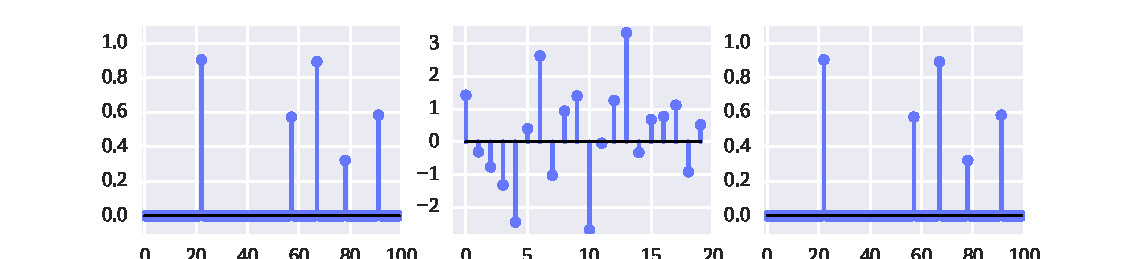
\includegraphics[width=\textwidth]{figs/figure_1h.pdf}
	\caption{\textit{Left}: The original $ 5 $-sparse vector $ x \in \R^{100} $. \textit{Center}: The sensed vector $ y \in \R^{20} $. \textit{Right}: Result of $ \ell_{1} $-minimization}
	\label{fig:l1min}
	\vspace{4pt}\hrule
\end{figure}





\subsection{Recasting \eqref{eq:P1} as a linear program}
Now that we have a tractable way of finding sparse solutions, we will look at one way to actually solve \eqref{eq:P1}. In this section we will see how one can use linear programming to do this. Linear programming (LP) is the study of problems on the form
\begin{equation}
	\maximize{\x\in\K^{N}} \c^{T}\x \quad \subjectto \A\x\leq\b~,~~ \x\geq\0
	\label{eq:LPgeneral}
\end{equation}
Thus, to use one of the algorithms developed for LP, we need to rewrite \eqref{eq:P1} as a linear program (ie, on the form \eqref{eq:LPgeneral}). 

In order to do this, three problems arise. Fist, we see from \cref{eq:LPgeneral} that LP problems do not take constraints on equality form, which is what we have in \eqref{eq:P1}. Second, LP problems only minimizes linear functions (ie, functions that can be written as a dot product between the solution vector and some constant vector). Absolute values, as we have in the $ \ell_{1} $ norm, can not be described this way. Third, a general LP problem requires all values in $ \x $ be non-negative. This is not a constraint we have in \eqref{eq:P1}.

We begin by addressing the first issue. This can be quite easily solved by observing that an equality constraint can be rewritten as two inequality constraints like so:
\[
	\A\z = \y \iff \A\z \leq \y \text{ and } \A\z \geq \y
\]

The second issue is a common one in LP. Thus there are also common ways to work around it. One popular way of doing this is to introduce new variables $ t_{i} $ for $ i \in \index{N} $ such that $ \abs{z_{i}} \leq t_{i} $ for all $ i $. Thus, 
\[ 
	\minimize{\z\in\Cx^{N}} \sum_{i=1}^{N} \abs{z_{i}}
\]
can be rewritten as
\[ 
	\minimize{\z,\mathbf{t} \in \Cx^{N}} \sum_{i=1}^{N}t_{i} \quad \subjectto \abs{z_{i}} \leq t_{i} \text{ for all } i \in \indexset{N}
\]
we can then rewrite the constraints as
\[
	\begin{array}{r l}
		z_{i} - t_{i} & \leq 0\\
		- z_{i} - t_{i} & \leq 0
	\end{array}
	\quad\text{for all } i \in \indexset{N}
\]
to arrive at the standard LP form. The $ t_{i} $'s are clearly non-negative since they are defined to be greater than or equal to an absolute value. 

The third issue is also a quite common one in LP. We now have two decision vectors, $ \z  $ and $ \mathbf{t} $, where the elements of $ \z $ does not need to be non-negative. We will solve this by introducing two new decision vectors $ \z_{+} $ and $ \z_{-} $, which will replace $ \z $ in the problem formulation. 

We define $ \z_{+} $ and $ \z_{-} $ as follows:
\[ 
	(\z_{+})_{i} = \twopartdef{z_{i}}{\text{if } z_{i} > 0}{0}{\text{otherwise}}
	\quad
	(\z_{-})_{i} = \twopartdef{-z_{i}}{\text{if } z_{i} < 0}{0}{\text{otherwise}}
\]
It is clear that $ \z = \z_{+} - \z_{-} $, it is also clear that $ \z_{+}, \z_{-} \geq \0 $. Substituting in $ \z_{+} - \z_{-} $ for $ \z $ in the original problem will then solve this issue. 

A final issue is that general LP problems concerns maximization problems, however \eqref{eq:P1} is a minimization problem. This is easily solved by observing that minimizing a function $ f $ is equivalent to maximizing $ -f $.

Combining all of the above we arrive at the LP formulation of basis pursuit:
\begin{equation}
%	\tag{P$_{1(LP)}$}
	\begin{array}{r r l l}
		\maximize{} & -\sum_{i=1}^{n} t_{i}         &          &  \\
		 \subjectto & \A\z_{+} - \A\z_{-}           & \leq \y  &  \\
		            & -\A\z_{+} + \A\z_{-}          & \leq -\y &  \\
		            & \z_{+} - \z_{-} - \mathbf{t}  & \leq \0  &  \\
		            & -\z_{+} + \z_{-} - \mathbf{t} & \leq \0  &  \\
		            & \z_{+}, \z_{-}, \mathbf{t}    & \geq \0   &
	\end{array}
\end{equation}
Thus, we can use all the celebrated algorithms for Linear Programming to solve \eqref{eq:P1}, such as the Simplex method, or various interior point methods \cite{vanderbei14linprog}.










\section{Good sensing matrices}
\label{sec:goodmatrices}
In this section we will look at the minimum number of measurements required, as well as some of the features we want our sensing matrix $ \A $ to possess, in order to ensure that basis pursuit works well. 

We will start by looking at how we can ensure unique $ s $-sparse solutions to the $ \ell_{1} $-minimization. Then we will look at how we can make sure that the solution to \eqref{eq:P1}, which is the problem we will solve in practice, is in fact the solution to \eqref{eq:P0}, which is the problem we actually want to solve. Finally we will look at which matrices will perform well with the different recovering algorithms used.





\subsection{Minimum number of measurements}
\label{sec:minimum_measurements}
In this section we will look at how many measurements we need in order to ensure that \eqref{eq:P0} has only one $ s $-sparse solution. We begin by stating the main result of this section:
\begin{theorem}
	\label{thm:minimum_measurements}
	If $ \set{\z \in \Cx^{N} \st \A\z = \A\x, \norm{\z}_{0} \leq s}  = \set{\x} $, that is, $ \x $ is the unique $ s $-sparse solution to \eqref{eq:P0}, then the number of measurements $ m $ must satisfy $ m \geq 2s $.
\end{theorem}

Before proving this theorem, we need the following lemma:
\begin{lemma}
	\label{lemma:uniquesol_linind}
	Every $ s $-sparse vector $ \x $ is the unique $ s $-sparse solution to \eqref{eq:P0} with $ \y = \A\x $ if and only if every set of $ 2s $ columns of $ \A $ is linearly independent.
\end{lemma}

We will not prove \cref{lemma:uniquesol_linind} in this report, but a proof can be found in \cite[Theorem~2.13]{foucart13intro}. We are now ready to prove the main result:
\begin{proof}[Proof of \cref{thm:minimum_measurements}]
	Assume that it is possible to uniquely recover any $ s $-sparse vector $ \x $ from the knowledge of its measurement vector $ \y = \A\x $. Then, by \cref{lemma:uniquesol_linind}, we have that every set of $ 2s $ columns of $ \A $ must be linearly independent. This implies that $ \rank \A \geq 2s $. From elementary linear algebra we know that the rank of a matrix can not be bigger that the number of rows, hence $ \rank \A \leq m $. Combining this, we get that
	\[
		2s \leq \rank \A \leq m
	\]
	which concludes the proof.
\end{proof}





\subsection{The Null Space Property}
\label{sec:NSP}
So far, we have only looked at the intuitive reasoning of why $ \ell_{1} $-minimization works well to find the $ \ell_{0} $-minimum. In this section we will formalize this relationship using the \textit{Null Space Property} (often abbreviated NSP). It can be shown that, for the NSP, the real and complex case are equivalent (for a formal statement and proof, see Theorem~4.7 in \cite{foucart13intro}). Hence we will state the definitions and results for a field $ \K $, which can be either $ \R $ or $ \Cx $. The NSP is defined as follows:

\begin{definition} \label{def:NSP}
	A matrix $ \A \in \K^{m\times N} $ is said to satisfy the \textit{null space property} relative to a set $ S \subset \indexset{N} $ if
	\[ 
		\norm{\v_S}_1 < \norm{\v_{\overline{S}}}_{1} \quad \forall ~ \v \in \ker \A \setminus \set{\0}
	\]
	It is said to satisfy the null space property of order $ s $ if it satisfies the null space property relative to any set $ S \subset \indexset{N} $ with $ \abs{S} \leq s $
\end{definition}

The definition of the NSP might seem a bit arbitrary, but as we will soon see, the NSP is directly connected to the success of basis pursuit. We begin by stating our first theorem on the NSP:

\begin{theorem}
	\label{thm:NSP_to_basis_special}
	Given a matrix $ \A \in \K^{m \times N} $, every vector $ \x \in \K^{N} $ supported on a set $ S $ is the unique solution to \eqref{eq:P1} with $ \y = \A\x $ if and only if $ \A $ satisfies the NSP relative to $ S $. 
\end{theorem}

\begin{proof}
	Proving equivalence amounts to proving two implications. We will begin by proving that if a vector $ \x $ supported on $ S $ uniquely solves \eqref{eq:P1}, then $ \A $ satisfies the NSP relative to $ S $.
	
	Given an index set $ S $, assume that every vector $ \x \in \K^{N} $ supported on $ S $ is the unique solution to
	\[
		\minimize{\z \in \Cx^{N}} \norm{\z}_1
		\subjectto \A\z = \A\x
		\tag{P$_1$}
	\]
	Since $ \ker\A $ is a subspace of $ \K^{N} $, it is clear that for any $ \v \in \ker\A\setminus\set{0} $, the vector $ \v_{S} $ is the unique solution to 
	\begin{equation}
		\label{eq:nspproofminprob}
		\minimize{\z \in \Cx^{N}} \norm{\z}_1
		\subjectto \A\z = \A\v_{S}
	\end{equation}
	Because $ \v \in \ker\A $, we have that $ \A\v = \0 $, which means that $ \A(\v_{S} + \v_{\overline{S}}) = \0 $, giving us that $ \A(-\v_{\overline{S}}) = \A\v_{S} $. Hence it clear that $ -\v_{\overline{S}} $ is also a feasible solution to \eqref{eq:nspproofminprob}, but since $ \v_{S} $ is assumed to be the \textit{unique} optimal solution to \eqref{eq:nspproofminprob}, we get that $ \norm{\v_{S}}_{1} < \norm{-\v_{\overline{S}}}_{1} $. Since $ \norm{\cdot}_{1} $ is a norm, we have that $ \norm{-\v_{\overline{S}}}_{1} = \abs{-1}\norm{\v_{\overline{S}}}_{1} = \norm{\v_{\overline{S}}}_{1} $ from \cref{def:norm}. Thus, we arrive at the following inequality:
	\[
		\norm{\v_{S}}_{1} < \norm{\v_{\overline{S}}}_{1}
	\]
	This establishes the NSP for $ \A $, relative to $ S $.
	
	To prove the other implication, assume first that the NSP holds for $ \A $, relative to a given set $ S $. Let $ \x $ be a vector in $ \K^{N} $ supported on $ S $. Let $ \z \in \K^{N} $ be a vector that satisfies $ \A\x = \A\z $, and assume that $ \x \neq \z $. Our goal will be to show that $ \norm{\z}_{1} $ must be strictly bigger than $ \norm{\x}_{1} $, which will prove the uniqueness of the solution. 
	
	Define $ \v = \x - \z $. Since $ \A\x = \A\z $, we have that 
	\[
		\0 = \A\x - \A\z = \A(\x -\z) = \A\v
	\]
	This means that $ \v \in \ker\A $. Since $ \x\neq\z $, we also have that $ \v\neq \0 $. If we use the triangle inequality of norms, as well as the definition of $ \v $, we obtain
	\[
	      \norm{\x}_{1} 
		= \norm{\x - \z_{S} + \z_{S}}_{1}
		  \leq \norm{\x - \z_{S}}_{1} + \norm{\z_{S}}_{1}
		= \norm{\v_{S}}_{1} + \norm{\z_{S}}_{1}
	\]
	Now, using the assumption that $ \A $ satisfies the NSP relative to $ S $ we get the next inequality
	\[
		\norm{\v_{S}}_{1} + \norm{\z_{S}}_{1} < \norm{\v_{\overline{S}}}_{1} + \norm{\z_{S}}_{1}
	\]
	Using the definition of $ \v $ and $ \z $ again, we arrive at our final result:
	\[ 
		  \norm{\v_{\overline{S}}}_{1} + \norm{\z_{S}}_{1}
		= \norm{\x_{\overline{S}} - \z_{\overline{S}}}_{1} + \norm{\z_{S}}_{1}
		= \norm{- \z_{\overline{S}}}_{1} + \norm{\z_{S}}_{1}
		= \norm{\z}_{1}
	\]
	This proves that $ \norm{\x}_{1} < \norm{\z}_{1} $ for any $ \z \in \K^{N} $ satisfying $ \A\x = \A\z $ and $ \x \neq \z $. This establishes the required minimality of $ \norm{\x}_{1} $, and thus the uniqueness of the solution.
\end{proof}

\cref{thm:NSP_to_basis_special} is not that interesting by itself, but if we let the set $ S $ vary, it immediately yields a more general result:

\begin{corollary}
	\label{thm:NSP_to_basis}
	Given a matrix $ \A \in \K^{m \times N} $, every $ s $-sparse vector $ \x \in \K^{N} $ is the unique solution to \eqref{eq:P1} with $ \y = \A\x $ if and only if $ \A $ satisfies the NSP of order $ s $. 
\end{corollary}

Before we prove this result, we will give a small remark: \cref{thm:NSP_to_basis} shows that if $ \A $ satisfies the NSP of order $ s $, the $ \ell_{1} $-minimization strategy of \eqref{eq:P1} will actually solve \eqref{eq:P0} for all $ s $-sparse vectors.

\begin{proof}[Proof of \cref{thm:NSP_to_basis}]
	Assume every $ s $-sparse vector $ \x\in\K^{N} $ is the unique solution to \eqref{eq:P1}. Then, for every set $ S $ with $ \abs{S} \leq s $ we can find a vector $ \x'\in\K $ supported on $ S $ which is the unique solution to \eqref{eq:P1}. By \cref{thm:NSP_to_basis_special} we then have that $ \A $ must satisfy the NSP relative to $ S $. Since this is true for all $ S $ with $ \abs{S} \leq s $, $ \A $ must satisfy the NSP of order $ s $.
	
	Conversely, assume that $ \A $ satisfies the NSP of order $ s $. Then, from \cref{def:NSP}, for every set $ S $ with $ \abs{S} \leq s $ we have that $ \A $ satisfies the NSP relative to $ S $. From \cref{thm:NSP_to_basis_special} we have that a vector $ \x\in\K^{N} $ is supported on $ S $ only if it is the unique solution to \eqref{eq:P1}. Since this is true for any set $ S $ with $ \abs{S} \leq s $, it is true for any $ s $-sparse vector.
\end{proof} 








\subsection{Coherence}
\label{sec:coherence}
Now that we know the minimum number of measurements needed for obtaining unique solutions, and the properties of $ \A $ needed to ensure that the solution to \eqref{eq:P1} is in fact the solution to \eqref{eq:P0}, we can start looking at how well the recovering algorithms will perform. In this section we will look at how the notion of \textit{coherence} can help us distinguish between matrices that will perform well with the different recovering algorithms, and which that will not. 

We want our reconstruction of $ \x $ to be fast and reliable. Since the $ i $'th element of our measurement vector $ \y $ is the inner product between the row $ i $ of $ \A $ and $ \x $, it makes intuitive sense that the columns of $ \A $ should be as ``scattered'' as possible. This leads us to the definition of coherence: 

\begin{definition}
	Let $ \A \in \Cx^{m\times N} $ be a matrix with $ \ell_{2} $-normalized columns $ \a_{1}, \a_{2}, \ldots, \a_{N} $. The \textit{coherence} $ \mu $ of $ \A $ is defined as
	\[
		\mu = \max_{1\leq i \neq j \leq N} \abs{\inner{\a_{i}}{\a_{j}}}
	\]
\end{definition}

It is worth noting that the coherence of a matrix $ \A $ is $ 0 $ if and only if $ \A $ is orthogonal. This agrees well with the intuitive approach discussed above. However, since compressive sensing deals with situations where $ m < N $, this will never be the case for any of the matrices we will look at. 

The question now becomes, how low can the coherence get? We know that we will never reach a coherence of $ 0 $, but how close can it be? The next lemma gives us a lower bound on the coherence:

\begin{lemma} \label{thm:welchbound}
	The coherence $ \mu $ of a matrix $ \A \in \K^{m \times N} $ with $ \ell_{2} $-normalized columns satisfies the following inequality:
	\[
		\mu \geq \sqrtl{\dfrac{N-m}{m(N-1)}}
	\]
\end{lemma}

\noindent This bound is often called the \textit{Welch bound}. The proof for this Lemma is rather technical, and will therefore be omitted from this report. A complete proof for \cref{thm:welchbound} can be found in \cite[Theorem~5.7]{foucart13intro}.

\todo[inline]{Eksempel med matriser med lav koherens?}







\section{Sparsity in the real world}
\subsection{Compressibility}
The general framework developed in \cref{sec:goodmatrices} is designed for \textit{sparse} vectors without any errors. What if our signal is almost sparse, but not quite? Or what if the sampled signal is slightly distorted? In this section we will briefly cover how we can extend the theory presented in \cref{sec:goodmatrices} to cover such cases.

In order to answer this precisely we first need to specify what we mean with \textit{almost sparse}. This is where the notion of compressibility comes in. A compressible vector is a vector where most entries is \textit{almost} zero. To more precisely define a compressible vector, we must first define what we mean by almost zero:
\begin{definition} \label{def:compressibility}
	For any $ p > 0 $, the $ \ell_{p} $-error of best $ s $-term approximation to a vector $ \x \in \Cx^{N} $ is defined by
	\(
		\sigma_{s}(\x)_{p} = \inf \set{\norm{\x - \z}_{p} : \z \text{ is } s\text{-sparse}}
	\)
\end{definition}

We say that a vector $ \x $ is $ s $-compressible if $ \sigma_{s}(\x)_{1} $ is small. The second potential issue we will cover is when our measured vector $ \y $ contains some noise, such that $ \A\x \approx \y $. If the distance between the distorted measurements $ \y $ and the real, unbiased signal $ \A\x $ is bounded by a parameter $ \epsilon $, we can rewrite the approximation constraint as $ \norm{\A\x - \y}_{2} < \epsilon $. This motivates the following variant of basis pursuit:
\begin{equation}
	\tag{P$_{1, \epsilon}$}
	\label{eq:P1eps}
	\minimize{\z\in\Cx^{N}} \quad\subjectto \norm{\A\z - \y}_{2} \leq \epsilon
\end{equation}
It can be shown that if the sensing matrix exhibits a strengthening of the NSP called \textit{robust NSP}, the error made by solving \eqref{eq:P1eps} is bounded by a weighted sum of $ \sigma_{s}(\x)_{1} $ and $ \epsilon $ \cite[Section~4.3]{foucart13intro}.



\subsection{Achieving sparsity or compressibility}
So far we have just assumed our solution vector $ \x $ to be sparse or compressible. However, most real life signals are rarely sparse. Images are usually not mostly black, and songs are usually not mostly silence. Hence, we need some way to represent natural signals in a sparse way. 

We will achieve this by applying what is known as a \textit{sparsifying transform}. Many such transforms exists, but in this report we will consider the \textit{Haar wavelet transform} as an example. The Haar wavelet is by far not the most efficient sparsifying transform, but it is quite understandable, which is why we have chosen it. 

The key idea in a wavelet transform is to take some object, expressed in a high resolution wavelet basis, and express it in terms of a lower resolution basis, and a detail basis. In the specific case of the Haar wavelet, those functions are defined as follows:
\[
	\phi(t) = \twopartdef{1}{\text{if } 0\leq t < 0}{0}{\text{otherwise}}
	\quad
	\psi(t) = \threepartdef{1}{\text{if } 0\leq t < 1/2}{-1}{\text{if } 1/2 \leq t < 1}{0}{\text{otherwise}}
\]
By shifting and scaling those functions we get a basis for the low resolution space (from the $ \phi $'s) and the detail space (from the $ \psi $'s). Since a digital image is piecewise linear in every pixel, it is clear that a digital image of size $ n \times n $ is in the $ n \times n $ dimensional high resolution resolution space for the Haar wavelet.

The Haar Discrete Wavelet Transform (Haar DWT) is essentially a change of coordinates from the higher resolution wavelet basis basis, to a lower resolution and detail basis. \cref{fig:dwt_sparsifying} illustrates what happens when the DWT is applied to an image. The upper left corner of the resulting image is the low resolution space. This is usually not any sparser or more compressible than the original image. However, in the upper right, lower left and lower right corners we see the detail space. This is highly compressible, and it is also clear that the total compressibility of the image has increased (ie, number of non-zero components has decreased). We will denote the corresponding matrix to this change of coordinates by $ \mathbf{\Psi} $. 

\begin{figure}[t]
	\centering
	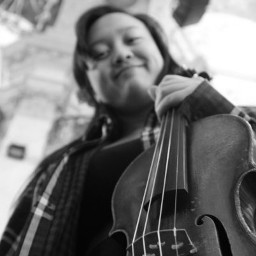
\includegraphics[width=0.47\textwidth]{figs/lily.jpg}
	\hspace{.039\textwidth}
	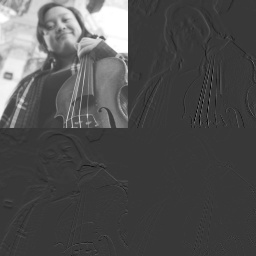
\includegraphics[width=0.47\textwidth]{figs/lily_wavelet.jpg}
	\caption{\textit{Left:} the original image of Lily. \textit{Right:} the image after a 1-level discrete wavelet transform using the Haar wavelet. In this example, we have used the 2D DWT implementation provided in \cite{ryan16applinalg}.}
	\label{fig:dwt_sparsifying}
	\vspace{4pt}\hrule
\end{figure}

We could assume that this change of coordinates have been done prior to the sensing, so that our solution vector $ \x = \mathbf{\Psi}\x' $ is sparse. Here $ \x' $ is the underlying non-sparse solution. However, we will instead include the change of coordinates in our sensing matrix $ \A $. Hence the sensing matrix becomes the following product:
\begin{equation}
	\label{eq:sensingmatrix_composition}
	\A = \mathbf{P}_{\Omega}\mathbf{\Phi}\mathbf{\Psi}^{-1}
\end{equation}
Here, $ \mathbf{P}_{\Omega} $ is a matrix describing the down-sampling, $ \mathbf{\Phi} $ denotes the sampling pattern used, and $ \mathbf{\Psi} $ is the basis in which $ \x $ is sparse. Typical choices include letting $ \mathbf{\Psi} $ be some wavelet basis, letting $ \mathbf{\Phi} $ be rows from the discrete Fourier matrix, and letting $ \mathbf{P}_{\Omega} $ pick out the first $ n $ rows.

This means that solving \eqref{eq:P1} results in a recovered vector $ \z $ also expressed in the $ \mathbf{\Psi} $-basis. To recover our real non-sparse vector $ \z' $ we would then have to apply the reversed change of coordinates:
\[
	\z' = \mathbf{\Psi}^{-1}\z 
\]
Since the columns of $ \mathbf{\Psi} $ form a basis, we know that the inverse $ \mathbf{\Psi}^{-1} $ exists by the Invertible Matrix Theorem.
%\cite[Theorem~2.8m]{lay16linearalgebra}


For ease of notation, we will simply refer to the sampling matrix as $ \A $, even though we think of it as a product of multiple matrices. The concepts we discussed earlier in \cref{sec:goodmatrices} will apply to this product $ \A $. We will also note that we will later use $ \mathbf{\Phi} $ to denote a matrix generated from training images. This is a different matrix, and should not be confused with the sampling pattern here. 






\chapter{Applications to Face Recognition} \label{sec:applications}
We will now shift our focus away from general compressive sensing, and look at how these techniques of sparse recovery can be used to build a framework for a complete face recognition system. 

The face recognition problem is a classical one in the area of statistical learning and machine intelligence. Hence it is a broadly studied problem, with many proposed solutions. The classical way to do face recognition is to first do what is called feature extraction. One can think of feature extraction as a projection to a lower dimensional feature space, such that the requirements for memory and computational power is reduced. Popular methods for this includes Principal Component Analysis and Discrete Cosine Transform \cite{bhat2014performance}.

After projecting the images down to a lower resolution space, one typically applies some statistical classification scheme. Typical classifiers used in classical face recognition include  Linear Discriminant Analysis (LDA) \cite{bhat2014performance}, $ K $ Nearest Neighbor/Subspace (KNN/KNS) \cite{lee2005acquiring} and (Linear-kernel) Support Vector Machines (SVM) \cite{wright09facerecog}. These methods seem to work well when in a controlled environment. However, when parameters such as lighting or noise level changes, or when a subject has occluded parts of his/her face (like the addition of glasses), these methods often begin to struggle \cite{eldar12theoryapplic}.

In this chapter we will introduce a new classification scheme called Sparse Representation-based Classification (SRC) \cite{wright09facerecog}. This is an alternative method to the LDA or KNN discussed above, but does not replace the dimensionality reduction. In this report, however, we will not discuss feature extraction in any more detail, but focus on the classification scheme. 

In order to do face recognition, we first need a set of $ N $ labeled \textit{training images} $ \set{(\phi_{i}, l_{i})}_{i=1}^{N} $. This is a set of images which our algorithm will use to learn what the different people we want to recognize looks like. Here, $ (\phi_{i}, l_{i}) $ denotes the tuple consisting of the $ i $'th image $ \phi_{i} $, and a label $ l_{i} \in \set{1, 2, \ldots, C} $ indicating which of the $ C $ subjects the image $ \phi_{i} $ is of. The task og the system is then, given a new test image $ \y $, to say which of the $ C $ subjects is pictured in $ \y. $




\section{Sparse Representation-based Classification} \label{sec:src}
At first we must address a potential problem. All of the theory developed in \cref{sec:basic_cs} concerns vectors in $ \K^{N} $, while we usually think of images as matrices in $ \R^{m\times n} $. It seems we have a problem with dimensionality. However this problem can be easily solved by simply stacking all the columns of the image matrix $ \A $ on top of each other in the following way:
\[
	\A = \begin{bmatrix}
		\a_{1} & \a_{2} & \cdots & \a_{n}
	\end{bmatrix} \in \R^{m\times n}
\]
becomes
\[
	\a = \begin{bmatrix}
		\a_{1}^{T} &
		\a_{2}^{T} &
		\cdots &
		\a_{n}^{T}
	\end{bmatrix}^{T} \in \R^{mn}
\]

We begin by making an observation: if our training images of subject $ i $ is of varying illumination, and if we assume that they are all aligned correctly, we will expect a test image of subject $ i $ to be closely approximated by a linear combination of the test images. That is, for a new test image $ \y $ of subject $ i $, there exists $ k_{i} $ coefficients $ c_{1}, c_{2}, \ldots, c_{k_{i}}  \in \R $ (here, $ k_{i} $ is the number of images of subject $ i $) such that:
\begin{equation}
	\label{eq:approxtestimage}
	\y \approx \sum_{j \st l_{j} = i} \phi_{j}c_{j}
\end{equation}We note that if we define $ \c_{i} \in \R^{k_{i}} $ to be the vector of all the coefficients, and $ \mathbf{\Phi}_{i} \in \R^{mn \times k_{i}} $ to be the matrix consisting of all the corresponding images as columns, we can rewrite \eqref{eq:approxtestimage} as:
\begin{equation}
	\label{eq:approxtestimagematrix}
	\y \approx \mathbf{\Phi}_{i}\c_{i}
\end{equation}
This is assuming that $ i $ is known, which of course it is not. However, we observe that we expect the test image to \textit{only} be a linear combination of the training images corresponding to the correct subject. This means that the coefficients corresponding to any other subject should be $ 0 $, or at lest very small. Thus we arrive at the zero-padded version of $ \c_{i} $:
\begin{equation*}
	\label{eq:c0def}
	\c_{0} = \begin{bmatrix}~\cdots & \0^{T} & \c_{i}^{T} & \0^{T} & \cdots~\end{bmatrix}^{T} \in \R^{N}
\end{equation*}
Now, if we concatenate all the images in the entire training database into a matrix as such:
\[
	\mathbf{\Phi} = \begin{bmatrix}\mathbf{\Phi}_{1} & \mathbf{\Phi}_{2} & \cdots & \mathbf{\Phi}_{C}\end{bmatrix} \in \R^{mn \times N}
\]
where $ \mathbf{\Phi}_{i} $ is the matrix consisting of all the training images of subject $ i $ concat\-enated, we see that we can rewrite \eqref{eq:approxtestimagematrix} as:
\begin{equation}
	\label{eq:approxtestimagefinal}
	\y \approx \mathbf{\Phi}\c_{0}
\end{equation}
This will clearly be the case, no matter what $ i $ is. 

Summarizing what we have shown so far, we get that we are given a sensed testing image $ \y $, and we are trying to find a vector of coefficients $ \c_{0} $ such that $ \y \approx \mathbf{\Phi}\c_{0} $. We also know that $ \c_{0} $ should be highly sparse, since we expect most images in the database to \textit{not} be similar to the testing image. In fact, we only expect an average of $ 1/C $ entries in $ \c_{0} $ to be non-zero. 

In the last chapter we introduced theory for finding the sparsest solution to such systems of equations. However, we now have a system of approximations. If we assume that the error is less than some error term $ \epsilon $, we can state a minimization problem that we expect $ \c_{0} $ to be the optimal solution to:
\begin{equation}
	\label{eq:cs_face_recog}
	\minimize{\c \in \R^{N}} \norm{\c}_{1} \quad\subjectto \norm{\y - \mathbf{\Phi}\c}_{2} \leq \epsilon
\end{equation}
We observe that \eqref{eq:cs_face_recog} has the same form as \eqref{eq:P1eps}. Thus, we can use compressive sensing techniques to solve this minimization problem. 

By finding an optimal solution to \eqref{eq:cs_face_recog}, we get a vector $ \hat{\c}_{0} $ of estimated coefficients. It remains to determine which person we believe the image to be of. We will do this by choosing the person who minimizes the squared error term. That is, the person $ i $ who minimizes the distance between the sampled test image $ \y $ and the linear combination of training images of person $ i $. In this respect, SRC can be thought of as a type of Nearest Neighbor. 

Summarizing all of the above, we get the algorithm described in \cref{alg:src}. 



\begin{algorithm}[tb]
	\caption{Sparse Representation-based Classification for face recognition}
	\label{alg:src}
	\begin{enumerate}
		\itemsep0em 
		\renewcommand{\parsep}{0pt}
		\renewcommand{\parskip}{0pt}
		\renewcommand{\itemsep}{0pt}
		\item[] \textbf{Input:} A matrix of training images $ \mathbf{\Phi} \in \R^{mn\times N} $ of $ C $ persons, a test image $ \y\in\R^{N} $, and a tolerance $ \epsilon > 0 $.
		\item Normalize the columns of $ \mathbf{\Phi} $ to have a $ \ell_{2} $ norm of $ 1 $
		\item Solve the $ \ell_{1} $-minimization problem:
		\begin{equation}
			\hat{\c}_{0} = \argmin_{\c} \norm{\c}_{1} ~\subjectto \norm{\mathbf{\Phi}\c - \y} \leq \epsilon
			\label{eq:src}
		\end{equation}
		\item Compute the residuals $ r_{i}(\y) = \norm{\y - \mathbf{\Phi}_{i}(\hat{\c}_{0})_{i}}_{2} $ for all $ i \in \indexset{C} $. Here $ \mathbf{\Phi}_{i} $ and $ (\hat{\c}_{0})_{i} $ denotes all the training images and estimated coefficients associated with person $ i $. 
		\item[] \textbf{Output:} $ \hat{l_{i}} $ = identity of $ \y = \argmin_{i} r_{i}(\y) $  
	\end{enumerate}
\end{algorithm}


\section{Addressing Corruption and Occlusion}
A common problem when dealing with numerical problems of any sort is the introduction of round-off errors. A typical computer today uses 64 bit processors, this means that the processor (and all the other components) can store and process 64 binary digits of a number. Any real number must then be approximated by the closest number possible to write with 64 binary digits. Typically, this introduces a small error $ \epsilon_{i} < 2^{-53} \approx 10^{-16} $ for every pixel in the image. In addition to round-off errors, all image sensors introduce some image noise. 

In addition to uniform noise, another problem we have to address is occlusion. A common problem with many of the classical face recognition systems is their incapability of dealing with occlusion. If a subject puts on a pair of sunglasses, let his/hers hair grow, cuts his beard, or so forth, an ideal system should still be able to classify the subject correctly.


\begin{definition}
	\label{def:propgrowth}
	We say a sequence of error-signal $ (\x, \mathbf{e}) $ exhibits \textit{proportional growth} with parameters $ \delta > 0 $, $ \rho \in (0,1) $, $ \alpha > 0 $ if	
	\[
		n = \lfloor \delta m \rfloor,\quad \norm{\mathbf{e}_{0}}_{0} = \lfloor \rho m \rfloor, \quad \norm{\x_{0}}_{0} = \lfloor \alpha m \rfloor
	\]
\end{definition}

Before we state the main result of this section, we will give an interpretation of the parameters involved in \cref{def:propgrowth}. Our first parameter, $ n $, gives a ratio between the length of the real signal, and the length of the measured signal. In other words, $ n $, is the compression rate. The next two parameters deals with sparsity: $ \alpha $ is a measure of the sparsity of the uncorrupted signal, and $ \rho $ is the sparsity of the error. 

If a signal exhibits this property, we have that the following result holds:

\begin{theorem}
	\label{thm:errorcorr}
	Fix any $ \delta>0 $, $ \rho<1 $. Suppose that $ \A $ is a random matrix with columns drawn independently from a multivariate normal distribution as such:
	\[
		\a_{i} \iid N\left(\boldsymbol{\mu}, \frac{\nu^{2}}{m}\mathbf{I}_{m}\right), ~ \norm{\boldsymbol{\mu}}_{2} = 1, ~ \norm{\boldsymbol{\mu}}_{\infty} \leq C_{\mu}m^{-1/2}
	\]
	for some constant $ C_{\mu} $. Assume that $ \nu $ is sufficiently small, that $ J \subset \indexset{m} $ is a uniform random subset of size $ \rho m $, that $ \boldsymbol{\sigma} \in \R^{m} $ with $ \boldsymbol{\sigma}_{J} $ $ \iid \text{Unif}(\set{-1, 1}) $ (independent of $ J $), that $ \boldsymbol{\sigma}_{\overline{J}} = \0 $ and that $ m $ is sufficiently large. Then with probability at least $ 1 - C e^{-\epsilon^{*}m} $ in $ A, J, \boldsymbol{\sigma} $, for all $ \x_{0} $ with $ \norm{\x_{0}}_{0} \leq \alpha^{*}m $ and any $ \mathbf{e}_{0} $ with signs and support $ (\boldsymbol{\sigma}, J) $, 
	\begin{align*}
		\label{eq:errorcorr}
		(\x_{0}, \mathbf{e}_{0}) = & \argmin_{(\x,\mathbf{e})} \norm{\x}_{1} + \norm{\mathbf{e}}_{1} \\
                          & \subjto \A\x + \mathbf{e} = \A\x_{0} + \mathbf{e}_{0}
	\end{align*}
	and the minimizer is uniquely defined.
\end{theorem}

The proof of this theorem is very technical, and will not be given here. It can be found in \cite{wright10dense}. We will instead give a small interpretation of its consequences. 

It is worth noting that many of the technical assumptions in \cref{thm:errorcorr} are present only to make the theorem provable.  The main result is that we can recover a signal by using $ \ell_{1} $-minimization, even if the signal has some noise, and even if the noise is not sparse. However, for this to work we need our error and signal to exhibit certain properties, and the most important one is the proportional growth. 

Intuitively, we can think of the result this way: If our error is very dense, we need the signal to be very sparse, and if our signal is dense, we need a sparse error in order for the recovering scheme to work. 

One last problem we will not look into is misalignment. Usually, images of faces are not perfectly aligned and cropped, so a fully functioning face recognition system should be able to deal with misaligned images. A more in-depth look at this can be found in Section~12.5 of \cite{eldar12theoryapplic}.










\chapter{Practical Implementation}
We now shift our attention away from the purely theoretical aspect, and towards the practical side. In this chapter we will seek to answer two main questions: How can a face recognition system using the SRC described in \cref{sec:src} be implemented? And how does it perform compared to the classical, state-of-the-art methods? We will begin by addressing the latter, and then look at some problems that arise when implementing the system.

In order to implement and test a face recognition system, one will need a database of faces to test on. Many such databases exists, and some include the CMU Multi-PIE, the Yale database (and its successor, the extended Yale B database) and the AR Face Database. 
\begin{table*}[t]
	\centering
	\renewcommand{\arraystretch}{1.2}
	\begin{tabular}{r | c c c c}
		& \multicolumn{4}{l}{\quad Feature dimension}                                 \\
		Classifier & $ \quad30\quad $ & $ \quad56\quad $ & $ \quad120\quad $ & $ \quad504\quad $ \\ \hline
		SRC & $ 0.125 $        & $ 0.083 $        & $ 0.060 $         & $ 0.035 $         \\
		NN & $ 0.229 $        & $ 0.165 $        & $ 0.128 $         & $ 0.093 $         \\
		NS & $ 0.110 $        & $ 0.096 $        & $ 0.081 $         & $ 0.066 $         \\
		SVM & $ 0.280 $        & $  0.150 $       & $ 0.060 $         & $ 0.023 $
	\end{tabular}
	\renewcommand{\arraystretch}{1}
	\caption{Test error rates reported in \cite{wright09facerecog} for the SRC, NN, NS and SVM using the Laplacian faces scheme for feature extraction, and using the extended Yale B database}
	\label{table:errorrates}
	\vspace{4pt}\hrule
\end{table*}

\section{Comparison with Classical Methods}
Now that we have introduced a new classifier for face recognition, an immediate question becomes: Why develop a new classification scheme based on compressive sensing when there already exists multiple statistical classifiers suitable for face recognition? 

In the field of statistical and machine learning, one studies, among other things, different classifiers, such as the LDA, KNN or SVM discussed earlier. Typically, we have that for one specific application, different classifiers will perform differently. Thus, for a given application, we can rate how the different classifiers perform. A common metric for classification performance is to observe the \textit{test error rate}.

In order to precisely test the accuracy of a classification model, we need some testing data independent from the training data. Typically, this is achieved by dividing the total data available into two sets: a training set used to build the model, and a test set used to test the model. For our case, we will split our set of images $ \set{(\phi_{i}, l_{i})}_{i=1}^{N} $ in two, and make sure that for each person $ i $, we have equally many images of $ i $ in the training and the testing set. In the rest of this section, we will by $ I \subset \indexset{N} $ denote the set of indices for the training images, and by $ J = \indexset{N} \setminus I $ denote the set of indices for the testing images. 

Given a model and a set of testing images, the \textit{test error rate} is given as
\begin{equation}
	\label{eq:errorrate}
	\dfrac{1}{\,\abs{J}\,} \, \sum_{i\in J} \mathcal{I}(\hat{l_{i}} \neq l_{i})
\end{equation}
where $ \hat{l_{i}} $ is the predicted label of the image, $ l_{i} $ is the true label of the image, and $ \mathcal{I} $ denotes the indicator function. A good classifier is one for which the test error rate is small \cite[Section~2.2]{ISLR}.

An empirical comparison of the SRC with the more classical methods NN (ie: KNN with $ K = 1 $), NS (KNS with $ K=1 $) and the linear-kernel SVM is found in \cite{wright09facerecog}. In this comparison, the researchers used the \textit{Extended Yale B Database} consisting of $ 2\,414 $ images of $ 38 $ individuals, as well as the \textit{AR database} consisting of over $ 4\,000 $ images of 126 individuals. For each subject, they used half of the images for training, and half of the images for testing. Then they paired up the different classifiers with different feature extraction and feature dimensions, and compared their test error rate\footnote{In \cite{wright09facerecog} they actually talk about the \textit{recognition rate}, which would be $ 1 - $ test error rate. My guess is that the authors are the \textit{``glass is half-full''}-kind of people.}.



We have included some of the results from \cite{wright09facerecog} in \cref{table:errorrates}. We have concentrated on the Laplacian faces scheme for feature extraction, as this seemed to perform well with all the different classifiers. As one can see from the table, the SRC performs quite well. It is also worth noting that the performance of the SRC varies less from the choice of feature extraction than compared to the other classifiers.

An even more impressive result appears when the different classifiers is applied to occluded or corrupted images. For images where parts of the face are occluded, the researchers found that the test error rate was below $ 0.02 $, even when up to $ 30\% $ of the face were occluded. At $ 40\% $ occlusion the test error rate increased to $ 0.1 $, and for $ 50\% $ they reported a test error rate of $ 0.35 $. Meanwhile, the researchers reported a test error rate of $ > 0.2 $ at $ 30\% $ occlusion for the nearest-neighbor methods, and at $ 50\% $ they reported a test error rate between $ 0.5 $ and $ 0.7 $. Similar results were found for corrupted images. 




\section{Performance Issues}
So far, we have only discussed the advantages of the SRC-based system for face recognition compared to the classical approaches. However, this gives an incomplete view of the system. In this section we will look at one major disadvantage to the SRC-based method, namely runtime and memory use. 

\subsection{Runtime Analysis}
We will begin by looking at how the runtime of \cref{alg:src} will increase as the size of the problem increases (ie, as $ C, N, m $ and $ n $ increases). To do this we will use the Big-O notation.
\begin{definition}
	Let $ f, g $ be two functions $ f, g\colon\N\to\R $. Then $ f(n) \in \bigo(g(n)) $ if there exists a $ c \in \R $ and a $ N \in \N $ such that $ f(n) \leq cg(n) $ for all $ n > N $.
\end{definition}
\noindent We can think of Big-O as an upper bound on the true runtime.

Step 1 and 3 of \cref{alg:src} are obviously linear-time operations. More precisely, they have a runtime of  $ \bigo(N) $ and $ \bigo(C) $ respectively. The bottleneck of the runtime is thus step 2. In \cref{sec:basisasLP} we saw how \eqref{eq:P1} could be recast as an LP problem. However, a famous result due to Klee and Minty renders this more or less useless. They showed that the Simplex method using the largest-coefficient pivoting rule uses $ \bigo(2^{n}) $ pivots worst case, where $ n $ is the number of decision variables \cite[Section~4.4]{vanderbei14linprog}. For our case this means that using the simplex method to implement \cref{alg:src} will have a worst case runtime of $ \bigo(2^{N}) $.

Various interior point methods exist, such as the path-following method. This algorithm uses Newton's method to iteratively find better and better approximations to the optimal solution. However, even though the number of iterations no longer has exponential growth, since each iteration typically uses $ \bigo(N^{2}) $ operations, this too is to slow for our case \cite[Section~12.6]{eldar12theoryapplic}. This is because in a real world example, we will a very large number of training images $ N $.

The last algorithm we will look at is the orthogonal matching pursuit used to create \cref{fig:l1min}. This algorithms solves a series of least-squares approximations. This too is an approach that scales badly, which is why it's mostly used for small problems \cite[Secion~3.2]{foucart13intro}.

It is worth noting that some optimization algorithms with better per-iteration runtime exists, such as the Augmented Lagrange multiplier method described in \cite[Alg.~12.2]{foucart13intro}. Other algorithms, such as homotopy algorithms, make use of the fact that the solution is sparse, and are able to recover the $ \ell_{1} $-minimum of an $ s $-sparse vector in $ \R^{N} $ in $ \bigo(s^{3} + N) $ time \cite{wright09facerecog}, which is a decent runtime. For a very sparse vector, this is close to linear-time. 



\subsection{Memory Usage}
As we now have seen, the issue with runtime can be somewhat dealt with. Still, another issue remains, and that is memory usage. 

Digital images without compression use a lot of disk space. A one megapixel gray-scale image, using 8 bits to encode the light intensity, will take up 1 megabyte of disk space. That in itself is not too much, but as the database of images grows, the sensing matrix $ \mathbf{\Phi} $ quickly becomes very large. For the extended Yale B database, consisting of over 2400 images, $ \mathbf{\Phi} $ takes up 1.2 gigabytes of disk space, assuming that we store the images in the discussed format, and that half of the available data is used for training. For the AR database this grows to roughly 2 gigabytes, and for the enormous CMU Multi-PIE database we will have a sensing matrix of over 350 gigabytes. 

It is clear that it is not feasible to allocate such matrices in memory. Hence we will need a way to multiply the matrix with a vector (as one needs to do in the constraints of the minimization problem in \eqref{eq:src}) without allocating the matrix. Results from numerical linear algebra tell us that in many cases it is possible to create a function which multiplies a vector with a matrix, without allocating the matrix in memory. A simple way to illustrate how we can avoid allocating the whole matrix is to notice that we only need one row at a time. Thus, we can allocate only $ N $ bytes of memory space, instead of $ mnN $. Better approaches exist, but we will not go into any more detail in this report. 

Feature extraction will also help. Typically, before constructing the database of training images, one applies one of the feature extraction schemes mentioned earlier. I this way we can reduce the size of each image down even as low as 120 pixels \cite[Section~12.2]{eldar12theoryapplic}.

Even though a combination of these techniques will help, the amount of data required for robust face recognition using the SRC classification scheme remains an issue. 







\chapter{Conclusions}
\todo[inline]{results, consequences, etc}


\printbibliography


\end{document}

